\providecommand{\main}{..}
\documentclass[\main/master.tex]{subfiles}
\begin{document}
\chapter{Methods and results}\label{chapter:Methods and results}

\section{System structure}
\subsection{Experiment setup}
\begin{figure}[htbp]
	\centering
	\fbox{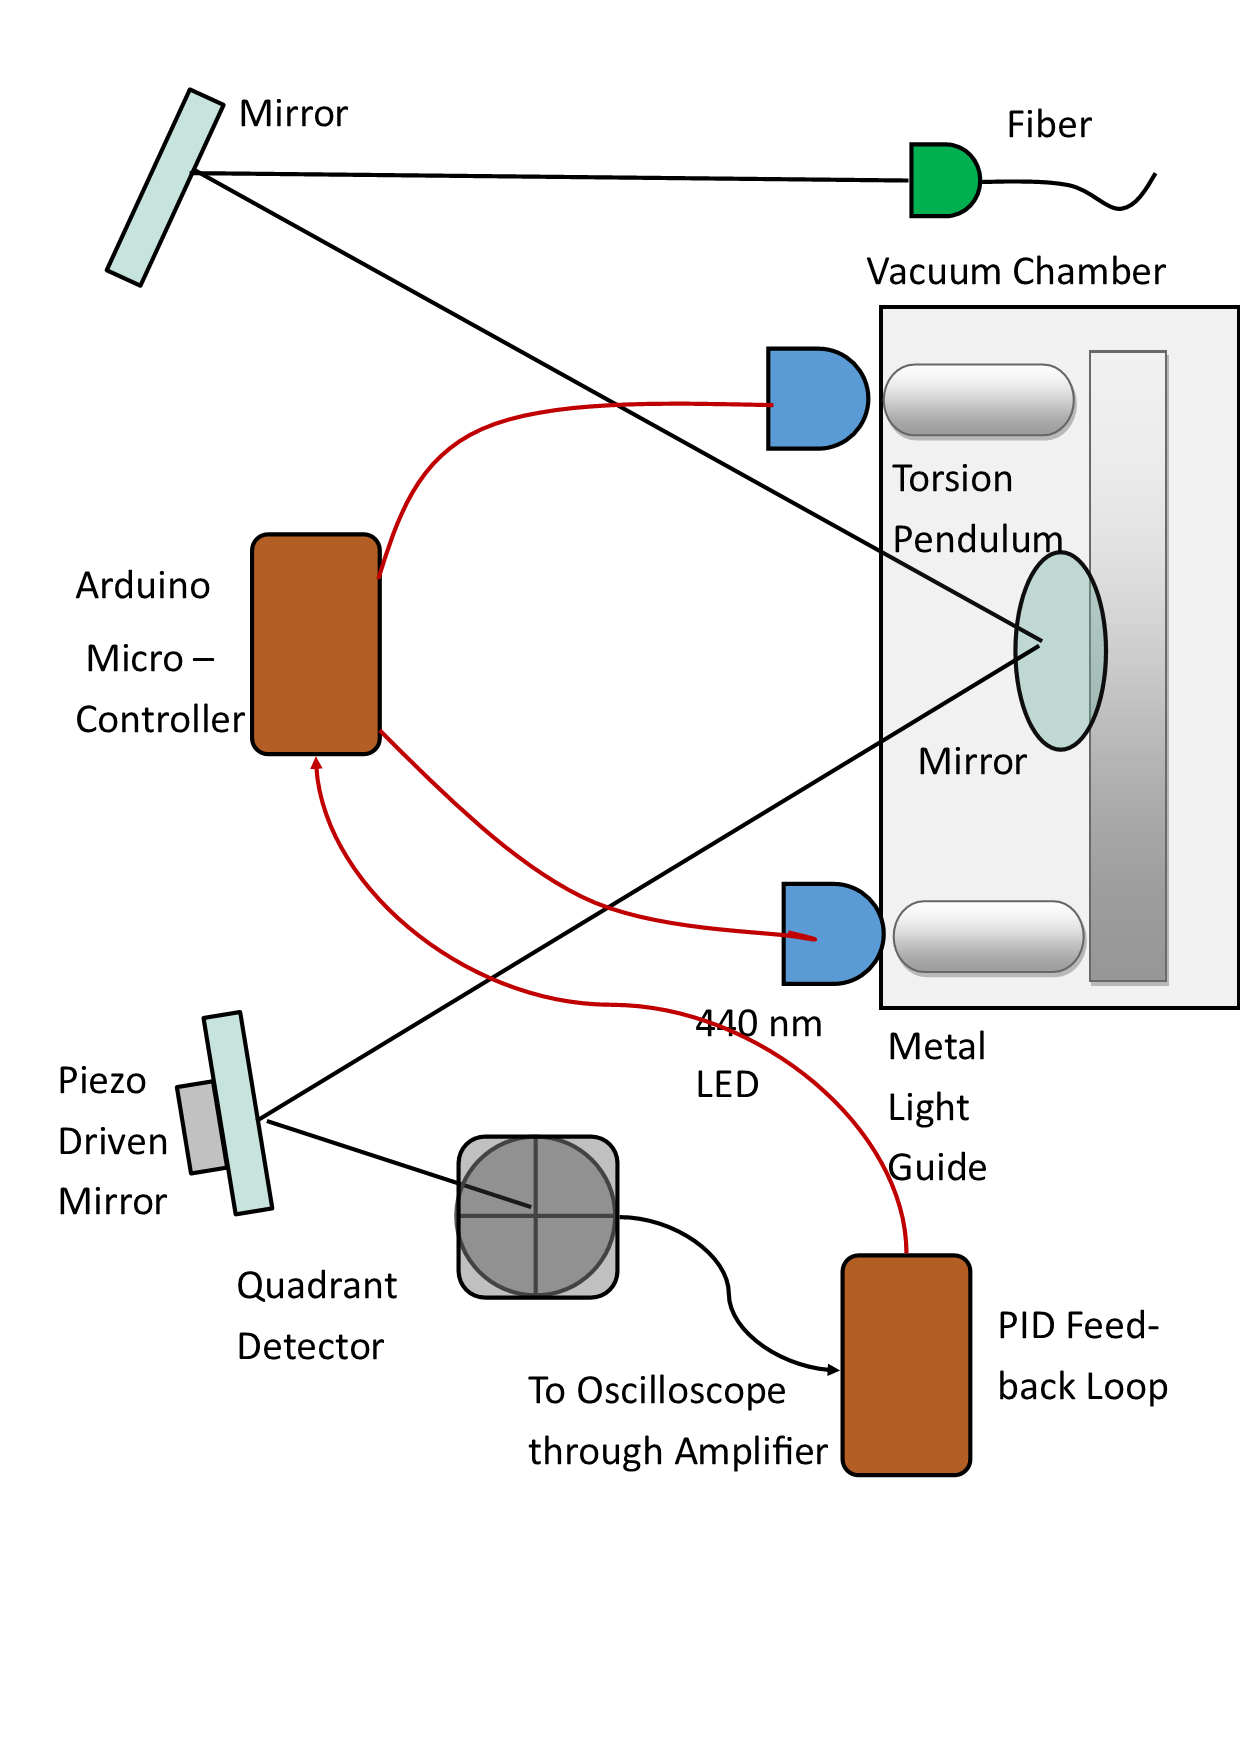
\includegraphics[scale=0.2]{\main/images/4 - methods and results/setup.png}}
	\caption[The experiment setup]{The experiment setup}
	\label{fig:setup}
\end{figure}
\FloatBarrier
\par\noindent
The experiment setup, shown in fig.~\ref{fig:setup}, is composed of a torsion pendulum placed inside a vacuum chamber, a tilt angle measurement system and a feedback system. The experiment setup is placed inside an acoustic box, which is not shown in the figure. The angle is measured by a laser beam deflected by the pendulum's front mirror and detected by a quadrant detector. The detector is connected to a computer by an oscilloscope through a signal amplifier. The light reflected from the pendulum mirror is reflected by a piezo driven mirror, which is tuned so that the reflected light would strike the detector's center (the PID needs a reference for error calculations). 
\par\noindent
The feedback system is composed of two LED light sources, modulated in real time by an Arduino micro-controller which is controlled by the PID feed-back loop in the computer. The LED light sources are each coupled to a side mass of the pendulum. The light is passed through the vacuum chamber by having transparent windows (viewports) on the sides of the chamber. 
\par\noindent
The vacuum chamber is connected to a vacuum engine, which is pumping out gas and lowering the pressure. When the desired pressure is achieved, the vacuum engine is disconnected using the valve and turned off, and the acoustic box is sealed. When the oscillations settle down to a level which could be affected by the weak torques caused by radiation pressure, the angle is read in real time by the PID algorithm, and radiation-pressure torque is exerted by the LED's flux for damping down the pendulum noises.
\subsubsection{Design of the system}
\begin{figure}[htbp]
	\centering
	\fbox{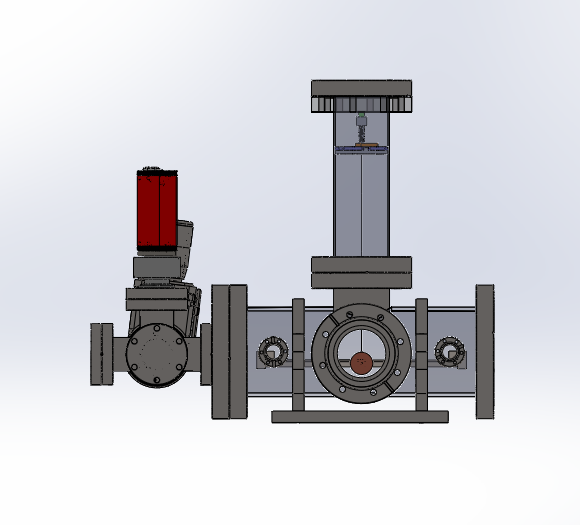
\includegraphics[scale=0.5]{\main/images/4 - methods and results/total_chamber.png}}
	\caption[Total chamber]{The system structure}
	\label{fig:Total chamber}
\end{figure}
\FloatBarrier
\par\noindent
The design of torsional pendulum and vacuum chamber, shown in fig.~\ref{fig:Total chamber}, was carried out using the software Solid Works. The torsional pendulum was manufactured by the university workshop, and the vacuum chamber was manufactured at HTC Vacuum. The assembling was performed at the HUJI lab. The system had undergone changes, and the final design of the system is presented. 
\par\noindent
As shown previously (eq.~\ref{eqn:drag force2}, eq.~\ref{eqn:total Brownian energy}, eq.~\ref{eqn:heat conduction}, eq.~\ref{eqn:acoustic power}), friction, Brownian motion energy, thermal power and acoustic waves are pressure dependent and are considerably reduced by maintaining low pressure. Therefore, the torsional pendulum is placed inside a vacuum chamber. Magnetic noise is reduced by choosing low magnetic permeability materials, avoiding capacitance and using a Faraday cage. 
\par\noindent
The vacuum chamber is placed inside an acoustic box, further reducing acoustic waves and magnetic noise. In order to maintain low pressure for long periods, the system is designed to minimize the outgassing rate by both, choosing low outgassing materials and avoiding air pockets inside the devices. 
\subsection{Vacuum chamber design}
\begin{figure}[htbp]
	\centering
	\fbox{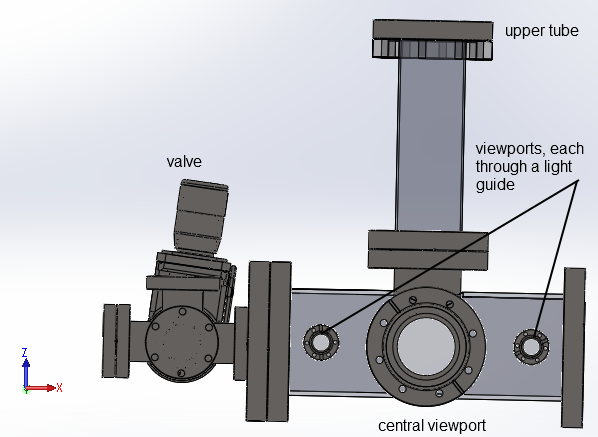
\includegraphics[scale=0.5]{\main/images/4 - methods and results/chamber_front_names.png}}
	\caption[Vacuum chamber, front view]{Vacuum chamber, front view}
	\label{fig:chamber front}
\end{figure}
\FloatBarrier

\par\noindent
The vacuum chamber, shown in fig.~\ref{fig:chamber front}, is composed of two cylindrical tubes placed one over the other with three view ports in front and light guides. The chamber is connected to a vacuum engine and gauge. The vacuum engine is connected to the chamber through a valve. The measurements are conducted when the valve is closed and the engine is off, to prevent rotation noise.

\subsubsection{Chamber viewports}
\par\noindent
The lower tube has three viewports. The central viewport is located in front of the pendulum's front mirror. The central viewport has a $68.3 [mm]$ view diameter where the mirror is located $82 [mm]$ away, giving a measurement FOV of about $39^0$ degrees. The other two small viewports are located in front of the pendulum's side masses and they are used for damping down the pendulum noises. They are connected to the chamber through light guides. The view ports are transparent for light in the $550-1100 [nm]$ range, with about 98$\%$ power transmittance in this range. 


\subsubsection{Vacuum maintenance}
\par\noindent
Due to the measurement sensitivity, the vacuum engine pumping must be off during measurement. Accordingly, the main limitations to the maintenance of low pressure are the leakage $Q_L$ from the outside (eq.~\ref{eqn:leak rate}) and the outgassing $Q_{des}$ inside the chamber (eq.~\ref{eqn:desorption rate}), thus increasing of the pressure at a constant rate over time. Due to the pendulum's shape and size, the vacuum chamber has large volume (high leak rate) and large surface area (high outgassing rate). 
\par\noindent
In order to minimize the pressure increase rate, the vacuum chamber is built using CF components which are designed for ultra high vacuum, and minimize the leak rate. Also, to reduce outgassing, the torsional pendulum and vacuum chamber were baked-out at $120 C^0$ for a week, using resistive wire. 
\par\noindent
The chamber volume is $V = 4.75\cdot 10^{-4}[m^3]$, and the measured pressure at the experiments after cooling down is $P \approx 1\cdot 10^{−2} [pa]$ for a month without pumping with the vacuum engine.
\subsection{Torsional pendulum design}
\subsubsection{Adjustable mount}
\begin{figure}[htbp]
	\centering
	\fbox{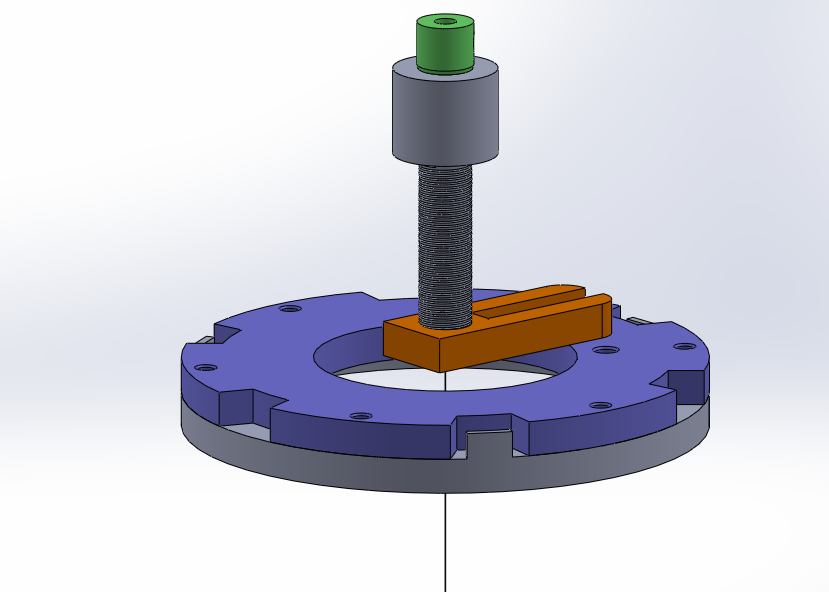
\includegraphics[scale=0.2]{\main/images/4 - methods and results/mount.png}}
	\caption[The pendulum mount]{The pendulum mount}
	\label{fig:mount}
\end{figure}
\FloatBarrier
\par\noindent
An adjustable mount for adjusting the height, distance and angle of the torsional pendulum, shown in fig.~\ref{fig:Total chamber}. The torsional pendulum string is held by the adjustable mount from the upper tube of the vacuum, placing it accurately in front of the viewports. 
\begin{figure}[htbp]
	\centering
	\fbox{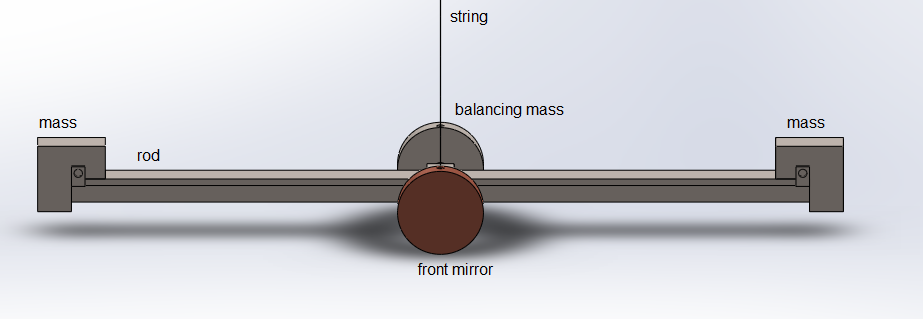
\includegraphics[scale=0.3]{\main/images/4 - methods and results/pendulum_front_names.png}}
	\caption[Torsional pendulum, front view]{Torsional pendulum, front view}
	\label{fig:pendulum front}
\end{figure}
\FloatBarrier
\par\noindent
The torsional pendulum design, shown in fig.~\ref{fig:pendulum front}, is composed of a thin rod with the length $2l$, string with the length $h$, two identical masses $m$ on the sides, a front mirror and a balancing mass to balance the center of mass. 
\begin{figure}[htbp]
	\centering
	\fbox{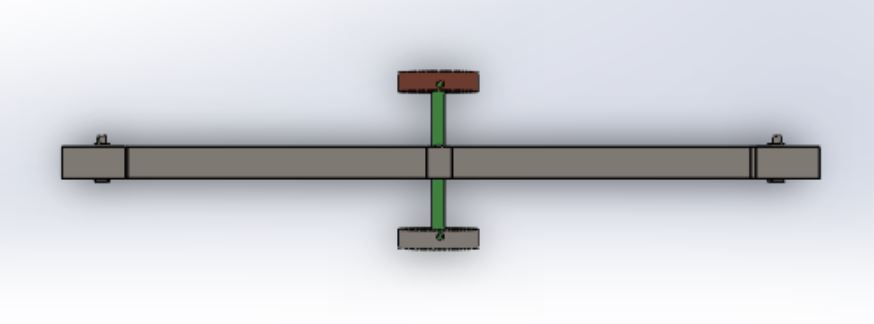
\includegraphics[scale=1.2]{\main/images/4 - methods and results/pendulum_top.JPG}}
	\caption[The torsional pendulum, top view]{The torsional pendulum, top view}
	\label{fig:pendulum top}
\end{figure}
\FloatBarrier 
\par\noindent
The center of mass is balanced using a balancing mass with similar shape and weight as the mirror on the other side, as shown in fig.~\ref{fig:pendulum top}. The balancing mass and the mirror are connected from their centers to the pendulum by a beam with length $w$, thus the overall downward torque $\tau_z$ with tilt angle $\phi$ is given by:
\begin{equation}
\tau_z = r_1\cdot m_1 g \cdot cos\phi - r_2\cdot m_2 g \cdot cos \phi\ = g\cdot cos\phi( m_1 r_1  - m_2 (w-r_1) )    \label{eqn:downward torque}
\end{equation}
Where $m_1$, $m_2$ are the masses of the mirror and the balancing mass, and $r_1$, $r_2$ are their distance from the pendulum's center of mass respectively. The beam allows to cancel out the torque $\tau_z$ by accurate adjustment of the distance $r_1$, given by: 
\begin{equation}
 r_1 = \frac{w}{\frac{m_1}{m_2}+1}  \label{eqn:downward torque cancelled}
\end{equation}


\subsubsection{Design constraints}
\par\noindent
The chosen pendulum dimensions are designed to achieve large angle sensitivity to the torque caused by a the gravity field (small string torsion coefficient $\kappa$ is needed, see eq.~\ref{eqn:theta average}) while maintaining large angle sensitivity to the measured mass (longer oscillation time period $T$, see eq.~\ref{eqn:theta average}). For a torsional pendulum with moment of inertia $I$ and string torsion coefficient $\kappa$, the oscillation time period $T$ is given by (eq.~\ref{eqn:undamped_omega}): 
\begin{equation}
T = 2\pi\sqrt{\frac{I}{\kappa}}  =  2\pi\sqrt{\frac{I}{\frac{G}{h} \frac{\pi d^4}{32}}}  \label{eqn:undamped_motion_equation_4}
\end{equation}
\par\noindent
According to eq.~\ref{eqn:undamped_motion_equation_4}, longer string length $h$ with smaller diameter $d$ results in small string torsion coefficient while having a large period time.
\par\noindent
The string is made of tungsten that is both, vacuum compatible (material with low outgassing) and has high tensile strength \cite{tungsten}, and is holding the pendulum robustly inside the vacuum chamber while having small string diameter. 
\par\noindent
In order to minimize the magnetic noise in the measurements, the torsional pendulum is made out of stainless steel 316 (instead of stainless steel 304) which has lower magnetic permeability \cite{SS316}, and the chosen front mirror is made fully of oxygen-free copper (OFC) instead of coated glass thus preventing capacitance. 
\subsubsection{Technical information}
The designed elements specifications are:
\begin{multicols}{2}
\raggedcolumns
\begin{easylist}
& Torsional beam;
&& Stainless steel 316.
&& length $2l=0.218 [m]$.
&& cross section $A =1.14\cdot10^{-2}[m^2]$.
&& mass weight $20.5\cdot10^{-3} [kg]$.
&& total weight $m_1=150\cdot10^{-3} [kg]$.
%& Mirror;
%&& OFC, gold coated.
%&& diameter of 1 inch.
\end{easylist}
\columnbreak
\begin{easylist}
& Tungsten string;
&& 99.95\% pure Tungsten
&& shear modulus $G = 130-160 [Gpa]$.
&& length $h= 0.249 [m]$.
&& diameter $d=80\cdot10^{-6}[m]$.
\end{easylist}
\end{multicols}
\subsection{Torsional motion}
The friction, Brownian motion, thermal flow and acoustic waves are reduced by having a lower pressure. The measurement system is placed inside an acoustic box, further reducing the acoustic power and also reducing magnetic noise as a Faraday cage. 
\par\noindent
The acoustic box is also a Faraday cage with 76 mm thickness, blocking magnetic fields with frequencies $f \ge 30 [Hz]$ from the environment. The vacuum chamber is a second cage that further blocks magnetic noise from the electronic system placed inside the acoustic box. The vacuum chambers is made out of approximately 3 mm thick stainless steel, blocking magnetic fields with frequencies $f\ge 20 [KHz]$ and reducing magnetic noise with lower frequencies.
\par\noindent
Initially the pendulum a driven oscillator (eq.~\ref{eqn:driven_motion_equation_2}) driven by small torques, consisted of black body radiation and pressure dependant noises. Gradually the pressure dependant friction (eq.~\ref{eqn:drag force1}) is damping the velosity, until the pendulum reaches an amplitude at which the friction is equal to the driving noises. The equilibrium amplitude is independent of the initial amplitude, but rather the pressure. After at least 8 hours of damping by the friction, the measured value is $\theta_{max}^{eq}\approx 1\cdot10^{-5}[rad]$. From the long damping time it can be shown the friction coefficient is very small, leading to a negligible friction at small amplitudes.
\par\noindent
As shown in eq.~\ref{eqn:Brownian uncertainty 3}, without noises the fundamental quantum uncertainty at room temperature results with an amplitude of  $\theta_{max}  \approx 4\cdot 10^{-8} [rad] $, meaning the pendulum noises  
\par\noindent
 
\par\noindent
\subsection{results}
The system measured results compared to the expected results from the equations are given by:
\begin{multicols}{2}
\raggedcolumns
\begin{easylist}
& expected;
&& $I = 0.487\cdot10^{-3}[kg\cdot m^2]$
&& $\kappa = 2.1\cdot10^{-6}[\frac{N\cdot m}{rad}] - 2.6\cdot10^{-6} [\frac{N\cdot m}{rad}]$
&& $T = 96[s] - 86 [s]$
\end{easylist}
\columnbreak
\begin{easylist}
& measured;
&& $\kappa = 2.7\cdot10^{-6}[\frac{N\cdot m}{rad}]$
&& $T = 84[s]$
&& $\theta_{max}^{eq} \approx 1\cdot10^{-5}[rad]$
\end{easylist}
\end{multicols}
The expected $\kappa$, $T$ have a range due to uncertainty of the string tensile strength $G$. The equilibrium amplitude $\theta_{max}^{eq}$ is an experimental value, depended on the amount of noise actually reduced, thus do not have an expected simulated value.



\section{Proportional–Integral–Derivative (PID) controller}
\subsection{Control stability}
The PID feed-back loop is continuously calculating the error value of the measured signal from a defined set point, which is the deviation of the pendulum amplitude from a $SP$ angle $e(t) =SP -\theta(t) $. The PID aims to reach the $SP$ with critical damping of the process (the torsional pendulum) by damping the error to zero. 
\par\noindent
In control theory there are two wanted conflicting properties; an accurate response (small overshoot), and small risetime (fast response). A PID control does not guarantee optimal control or stability of the process. When PID not tuned correctly, it can either overshoot or have a slow response, both resulting with a driven oscillator. The PID response to error (shown in eq.~\ref{eqn:PID response}) defines how much will the oscillator overshoot the $SP$.
\par\noindent
Overshoot is when the value of output signal (the actual response) exceeds the target value (the wanted response), thus the response is not accurate. The overshoot of a second order system is given by:
\begin{equation}
overshoot =  \frac{output-target}{target} = e ^{\frac{-\xi\pi}{\sqrt{1-\xi^2}}}  \label{eqn:overshoot}
\end{equation}
\par\noindent
Where $\xi$ is the damping ratio of the oscillator defined in eq.~\ref{eqn:system damping ratio}. As seen in eq.~\ref{eqn:overshoot} when the PID gains are too high, instead of critical damping there is overdamping, which is causing overshoot. Due to the high gains the overshoot response overshoots again to the other side, causing the system to be an unwanted driven oscillator (shown in eq.~\ref{eqn:driven_motion_equation_2}). A slow response causes phase delay between the signal and the equivalent PID response, resulting  again with a driven oscillator.
\subsection{Damped oscillator}
The torsional pendulum is a simple harmonic oscillator with oscillations amplitude $\theta_{max}$ and velocity given by $\dot{\theta}(t) =\frac{2\pi}{T} \theta_{max}( t)$ (see eq.~\ref{eqn:undamped_motion_equation_solved}). 
\par\noindent
The PID mainly acts as friction, gradually working when the oscillations are at the maximum velocity slowing them down, with a torque $\tau_{PID}$ given by:
\begin{equation}
\tau_{PID}(t) = -\gamma\dot{e}(t) =  -\gamma\cdot [\dot{SP} -\dot{\theta}(t)] =-\gamma\cdot [0-\dot{\theta}(t)]  =  \gamma\dot{\theta}(t) =  \gamma\frac{2\pi}{T} \theta_{max}( t) 
\label{eqn:friction_torque_pid}
\end{equation}
\par\noindent
Where $\gamma$ is the PID damping coefficient (eq.~\ref{eqn:damped_motion_equation}). Accordingly, the PID damping coefficient $\gamma$ is given by:
\begin{equation}
\gamma  =  \frac{\tau_{PID}(t)}{\frac{2\pi}{T} \theta_{max}( t) } =\frac{\tau_{max}}{\theta_{max}}\cdot \frac{ T}{2\pi}          \label{eqn:pid damping coefficient}
\end{equation}
Where $\tau_{max}$ is the maximal torque exerted by the PID. When damping using the PID the damping type, defined by the damping ratio $\xi$, and the damping time $\tau$ are given by (eq.~\ref{eqn:damping_time}):
\begin{equation}
\xi = \frac{T}{2 \pi \tau } =  \frac{T}{2 \pi  }\frac{\gamma}{2I} =\frac{T}{2 \pi  }\frac{\gamma}{2I} = \frac{ \tau_{max}}{\theta_{max}} \cdot \frac{T^2}{8\pi I}  \label{eqn:damping_time_pid}
\end{equation}
The PID damping $\gamma$, the damping time $\tau$ and the damping type defined by $\xi$ depend on the ratio $\theta_{max}/\tau_{max}$. If $\theta_{max}$ is too large compare to the external torque, the PID affect is negligible, resulting with a highly underdamped oscillator with infinite damping time. 
\par\noindent
In order to succeed in damping the pendulum, the PID must be able to exert torques which can critically damp the equilibrium amplitude (eq.~\ref{eqn:critically_damped_motion_equation}). The PID maximal torque $\tau_{max} $ is given by:
\begin{equation}
\tau_{max} (\xi = 1)\geq\frac{ 8 \pi I }{T^2}\cdot\theta_{max}^{eq} = \frac{  8 \pi \cdot 0.487\cdot10^{-3} }{(84)^2}\cdot 1\cdot10^{-5} = 1.7\cdot10^{-11}[N\cdot m]
\label{eqn:damping_torque_pid}
\end{equation}
\par\noindent
In order to damp the torsional pendulum the PID maximal torque is given by eq.~\ref{eqn:damping_torque_pid}. Since, the torque is proportional to the oscillations velocity (eq.~\ref{eqn:friction_torque_pid}), it needs a high modulation rate compare to the oscillations period $T$ (to prevent phase delay), and high dynamic range compare to velosity amplitude $\dot{\theta}_{max}$ (to avoid overshoot). 
%The sufficient modulation speed and range are unknown.
\subsection{Radiation-pressure torque}
The PID torque was chosen to be a Radiation-pressure torque. The setup is composed of two light sources with given flux, $\Theta_i(t)$, one in front of a mass on a side of the torsional pendulum. As seen in eq.~\ref{eqn:net_gravitation_torque}, the difference between two torques adds an external net torque. Assuming that both light fields have the same coupling efficiency $\eta$ and are very close to be perpendicular to the surface with negligible incidence angles $\alpha_1\approx\alpha_2\approx 0$, using eq.~\ref{eqn:radiation_force_power}, the radiation-pressure net torque $\tau(t)$ can be calculated by:  
\begin{equation}
\tau(t) = l\cdot F_1(t) \cdot cos\alpha_1 - l\cdot F_2(t) \cdot cos\alpha_2\approx l(F_1(t) - F_2(t)) \approx \frac{2l\eta}{{c}} \Delta \Theta(t) \label{eqn:radiation torque}
\end{equation}
The radiation-pressure net torque can be controlled by changing the difference between the light sources' flux $\Delta \Theta(t)$. Thus, the maximal net torque $\tau_{max}$ is given by: 
\begin{equation}
\tau_{max}  \approx \frac{2l\eta}{{c}} \cdot 2 \Theta_{max} \approx \frac{0.218\cdot \eta}{{3\cdot10^{8}}} \cdot 2 \Theta_{max} \approx 7.27\cdot10^{-10} \cdot \eta\Theta_{max}   \label{eqn:max radiation torque}
\end{equation}
Where $\Theta_{max}$ is the is the the light sources' maximal flux with optical setup efficiency $\eta$. 
\subsection{Laser setup}
Initially the modulated light sources were composed of a single laser diode coupled in series into two acousto optic modulators (AOM), with special filtered mode using optical fibers. The AOMs divides the single coherent light beam into two beams, with both the total power and the intensity ratio modulated the a response to input voltage, resulting with controlled modulation of the light sources difference.
\par\noindent
The apparatus had dynamic range of 1000 steps and modulation speed of $1 sec$. The setup minimized uncertainties of the light intensity since both light sources had a mutual source, partly cancelling internal noises such as thermal and shot noise. 
\par\noindent
The apparatus uncertainty due to the non linearity of the AOM response and laser power fluctuations proved to be larger than the uncertainties of the intensity difference. Also, modulation speed (response time) proved to be more important than modulation range. Due to the conclusions, the PID torque was changed to two controlled high power Light emitting diode (LED) sources.
\subsection{Light emitting diode (LED)}
The light emitting diode (LED) is a semiconductor light source with high power, and a long lifetime. A forward voltage applied to a p-n junction, causes electron injection which recombine with holes. The recombination releases energy in form of spontaneous emission photons (incoherent light). Due to the electrons life time, the LED could be modulated up to $100MHz$ (fast response, which can minimize the PID phase delay). Given by the Shockley diode equation for p-n junctions, the LED forward voltage $V_l$ is:
\begin{equation}
V_l(I_l) \approx n V_T ln10 log_{10} (\frac{I_l}{I_s})\approx constant \label{eqn:led voltage}
\end{equation}
Where $I_l$ is the LED current, $I_s$ is the saturation current, $n$ is the emission coefficient, and $V_T$ is the thermal voltage. Since the forward voltage varies as the logarithm of the current, it varies slowly, being approximately constant over wide current range, resulting with large changes in the LED current due to small changes in the circuit supply voltage $V$. In the driving circuit a resistor $R$ is connected in series with the LED to stabilizes the current, The LED flux with circuit of $N$ voltages supplies in parallel is given by:
\begin{equation}
\Theta = I_l\cdot V_l  =\frac{N\cdot V-V_l}{R}\cdot V_l\approx \frac{N\cdot V_l\cdot V}{R}\label{eqn:led power}
\end{equation}
\par\noindent
The LED light source has approximately a linear response (see eq.~\ref{eqn:radiation torque}) which can minimize the PID overshoot.
\par\noindent
The LED illumination angle varies between $45^0-120^0$. Since emitted light is incoherent it is hard to focus it to a point (not diffraction limited) and it has wide bandwidth spectrum. In order to overcome the LED incoherent profile and large illumination angle, the LED light sources are coupled to light guides (the vacuum chamber viewports were designed to have light guides in front). A light guide is a pipe made of thin filaments causing internal reflections, designed to illuminate small areas, regardless of the spectral characteristics of the light source. The light guide efficiency $\eta$ is mainly dependent on the cross section and length of the lightguide, making it ideal to overcome focusing problems. 


\subsection{Arduino microcontroller}
The modulated light sources are two LED light sources driven by an Arduino microcontroller, causing the PID torque. The Arduino is an inexpensive open-source microcontroller with a serial communication interface and a digital output without digital-to-analog converter (DAC). The Arduino Mega 2560 contains ATmega2560 8-bit controller, a $16 [MHz]$ crystal oscillator (clock) and 15 PWM outputs pins with digital output of $V_d = 5[V]$.
\begin{figure}[htbp]
	\centering
	\fbox{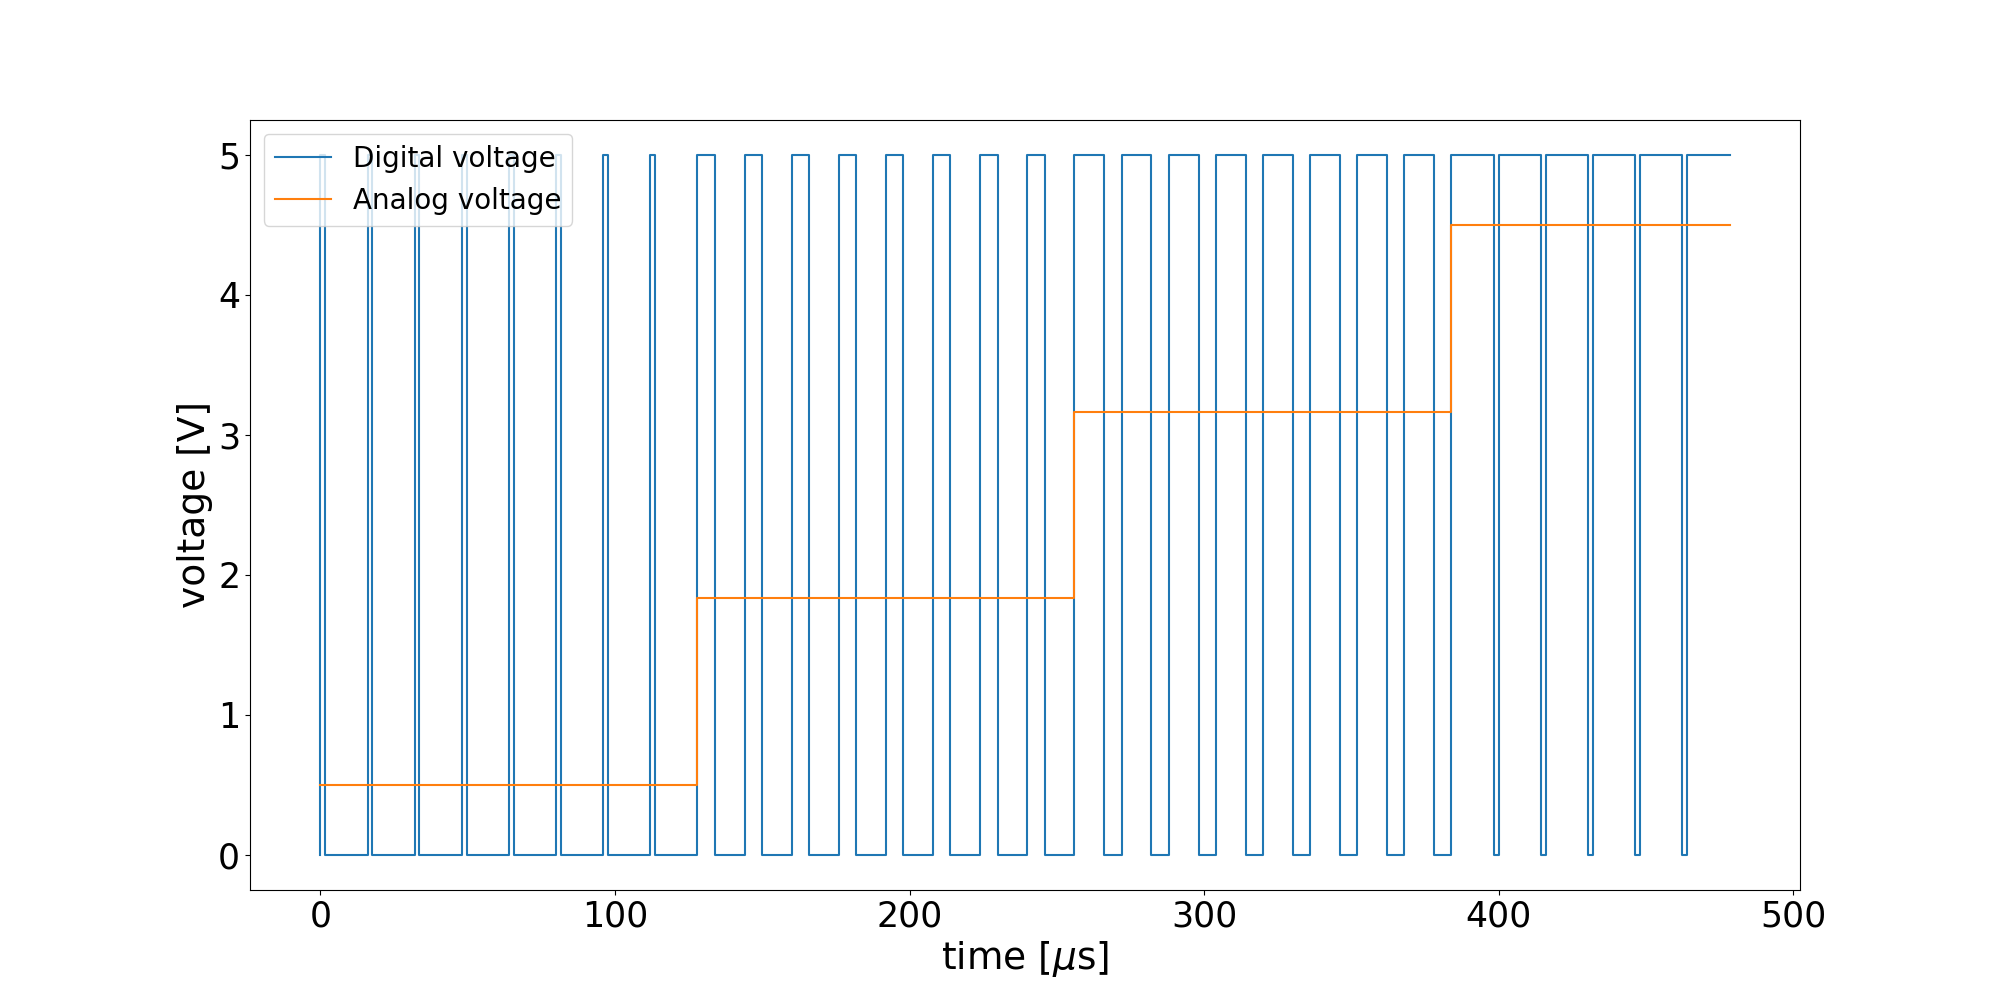
\includegraphics[scale=0.17]{\main/images/4 - methods and results/duty_cycle.png}}
	\caption[The PWM analog voltage]{The PWM analog voltage}
	\label{fig:duty_cycle}
\end{figure}
\FloatBarrier
\par\noindent
The microcontroller can simulate analog output using Pulse Width Modulation (PWM). As shown in fig.~\ref{fig:duty_cycle}, the controller switches the output signal on and off, generating a square wave with period $T$. Pulse width ($PW$) is the time duration in which the signal is on, the controller is able to modulate the $PW$, and thus change the duty cycle which is the ratio of time signal is on compared to off $D(t) = \frac{PW(t)}{T}\cdot 100$. The duty cycle varies between $0-100$, with resolution limited by the controller. The modulation is proportional to the analog average voltage $V_a$ given by: 
\begin{equation}
V_a(t) = \frac{ PW(t)\cdot V_d}{ T}  = \frac{V_d}{100}\cdot D(t)   \label{eqn:pwm voltage}
\end{equation}
Since the Arduino clock is connected to all PWM pins, they are all synchronized and have the same voltage, frequency and phase, allowing to connect them in parallel. The clock must have at least 120 periods of square waves before it can change to a new duty cycle value, this limits the voltage modulation frequency. Another limitation to the duty cycle change rate is the controller bit-rate. Accordingly, PWM maximal frequency is given by:
\begin{equation}
f_{PWM} = \frac{1 }{120T}= \frac{1 }{120 \frac{8-bit }{16MHz}}  \approx 500[Hz]	    \label{eqn:pwm frequency}
\end{equation}

\subsection{LED circuit}
The LED circuits are each composed of a blue LED with $V_l\approx 4.5V$, with $N=6$ parallel PWM Arduino pins for the supply voltage (eq.~\ref{eqn:pwm voltage}) and resistor $R = 200\Omega$. Due to coupling efficiency and size difference between the output beam from the lightguide and the pendulum sides, the efficiency of flux hitting the pendulum is estimated $\eta = 0.7$, thus with LED flux given by eq.~\ref{eqn:led power}, the PID torque $\tau_{PID}(t)$ is given by (eq.~\ref{eqn:radiation torque}):
\begin{equation}
\tau_{PID}(t) \approx \frac{2l\eta}{{c}} (\Theta_1(t) -\Theta_2(t)) \approx \frac{2l\eta}{{c}} \cdot\frac{N V_l V_d}{100R}(D_1(t) -D_2(t))  \approx   3.4\cdot 10^{-12}(D_1(t) -D_2(t)) 
\label{eqn:led torque}
\end{equation}
\par\noindent
The torque is controlled by the duty cycle $D(t)$ varying between $0-100$ with 8bit resolution, thus generating torques up to $\tau = 6.8\cdot10^-{10} [N\cdot m]$ with modulation steps of $\Delta\tau = 1.34\cdot10^-{12} [N\cdot m]$ and modulation frequency up to $500[Hz]$ (see eq.~\ref{eqn:pwm frequency}).
\section{Results and analysis} 
\subsection{Results}

\begin{figure}[htbp]
	\centering
	\fbox{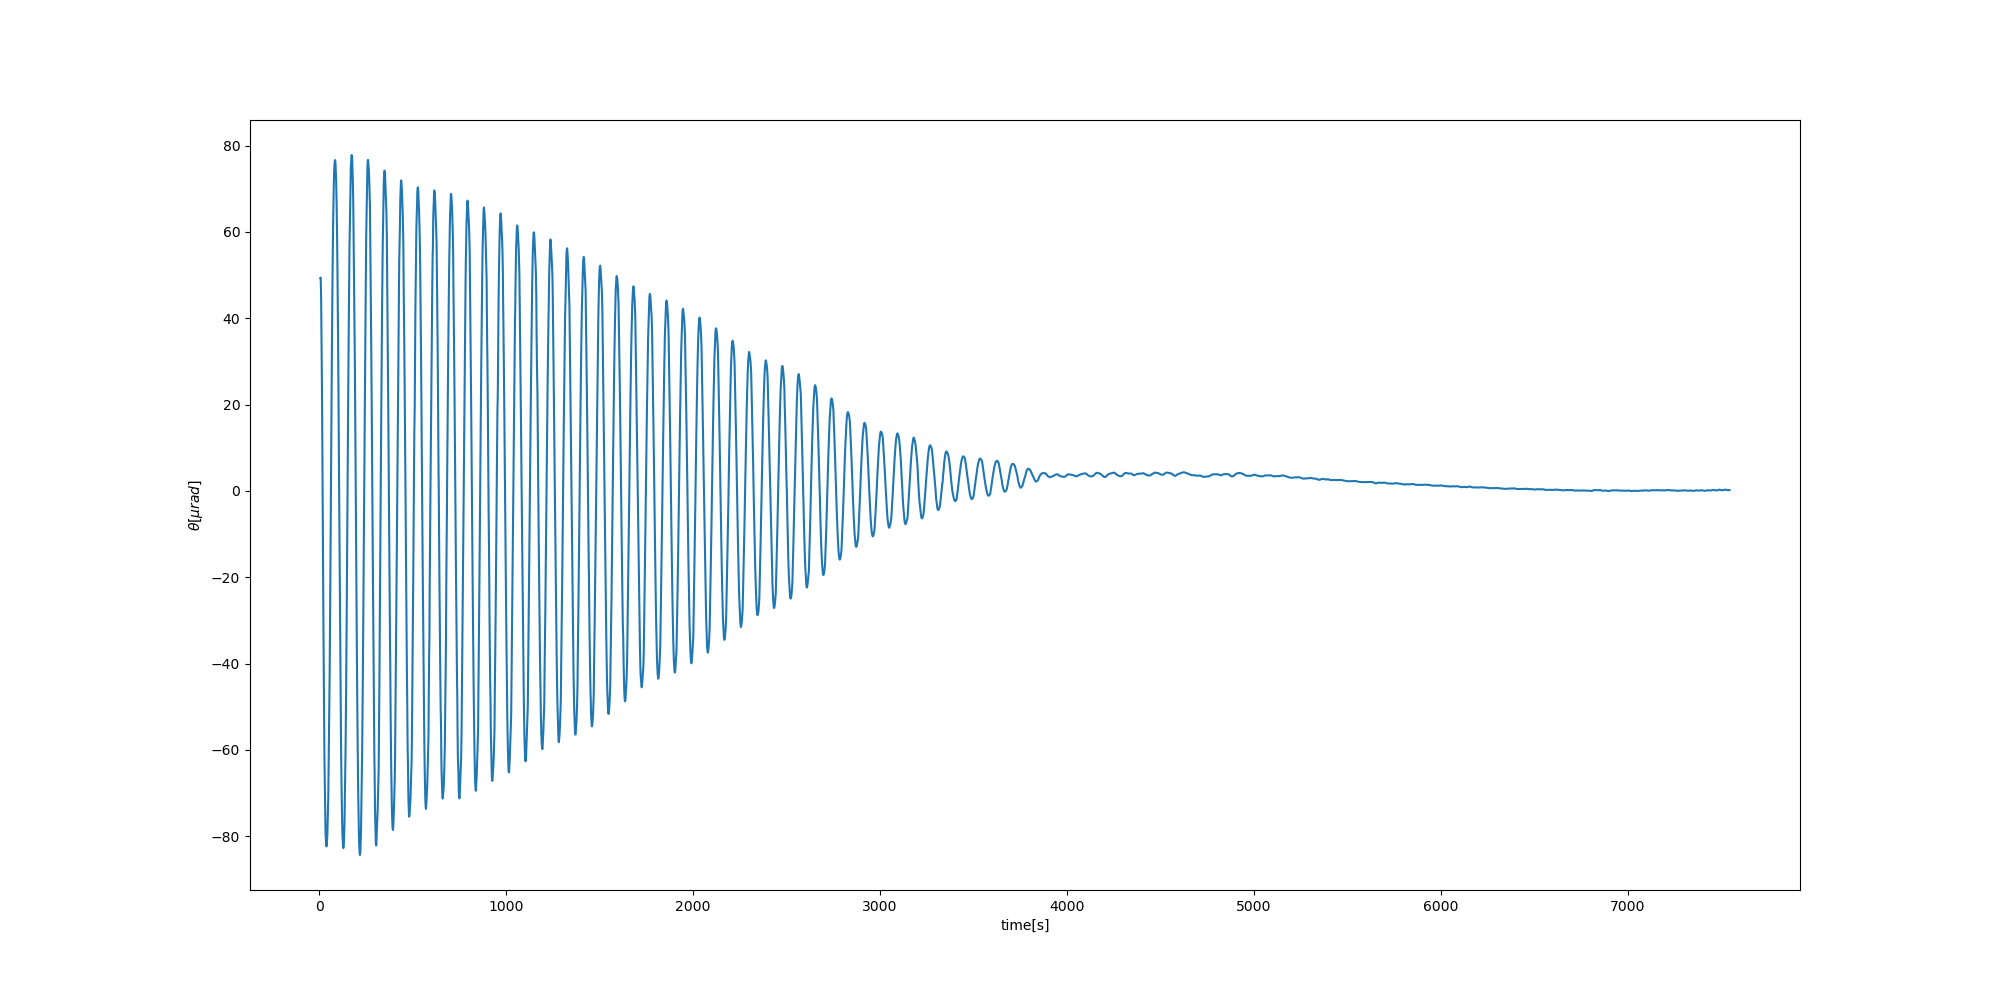
\includegraphics[scale=0.17]{\main/images/4 - methods and results/measured oscillation angle.png}}
	\caption[The damped torsional pendulum oscillations]{The damped torsional pendulum oscillations}
	\label{fig:measured oscillation angle}
\end{figure}
\begin{figure}[htbp]
	\centering
	\fbox{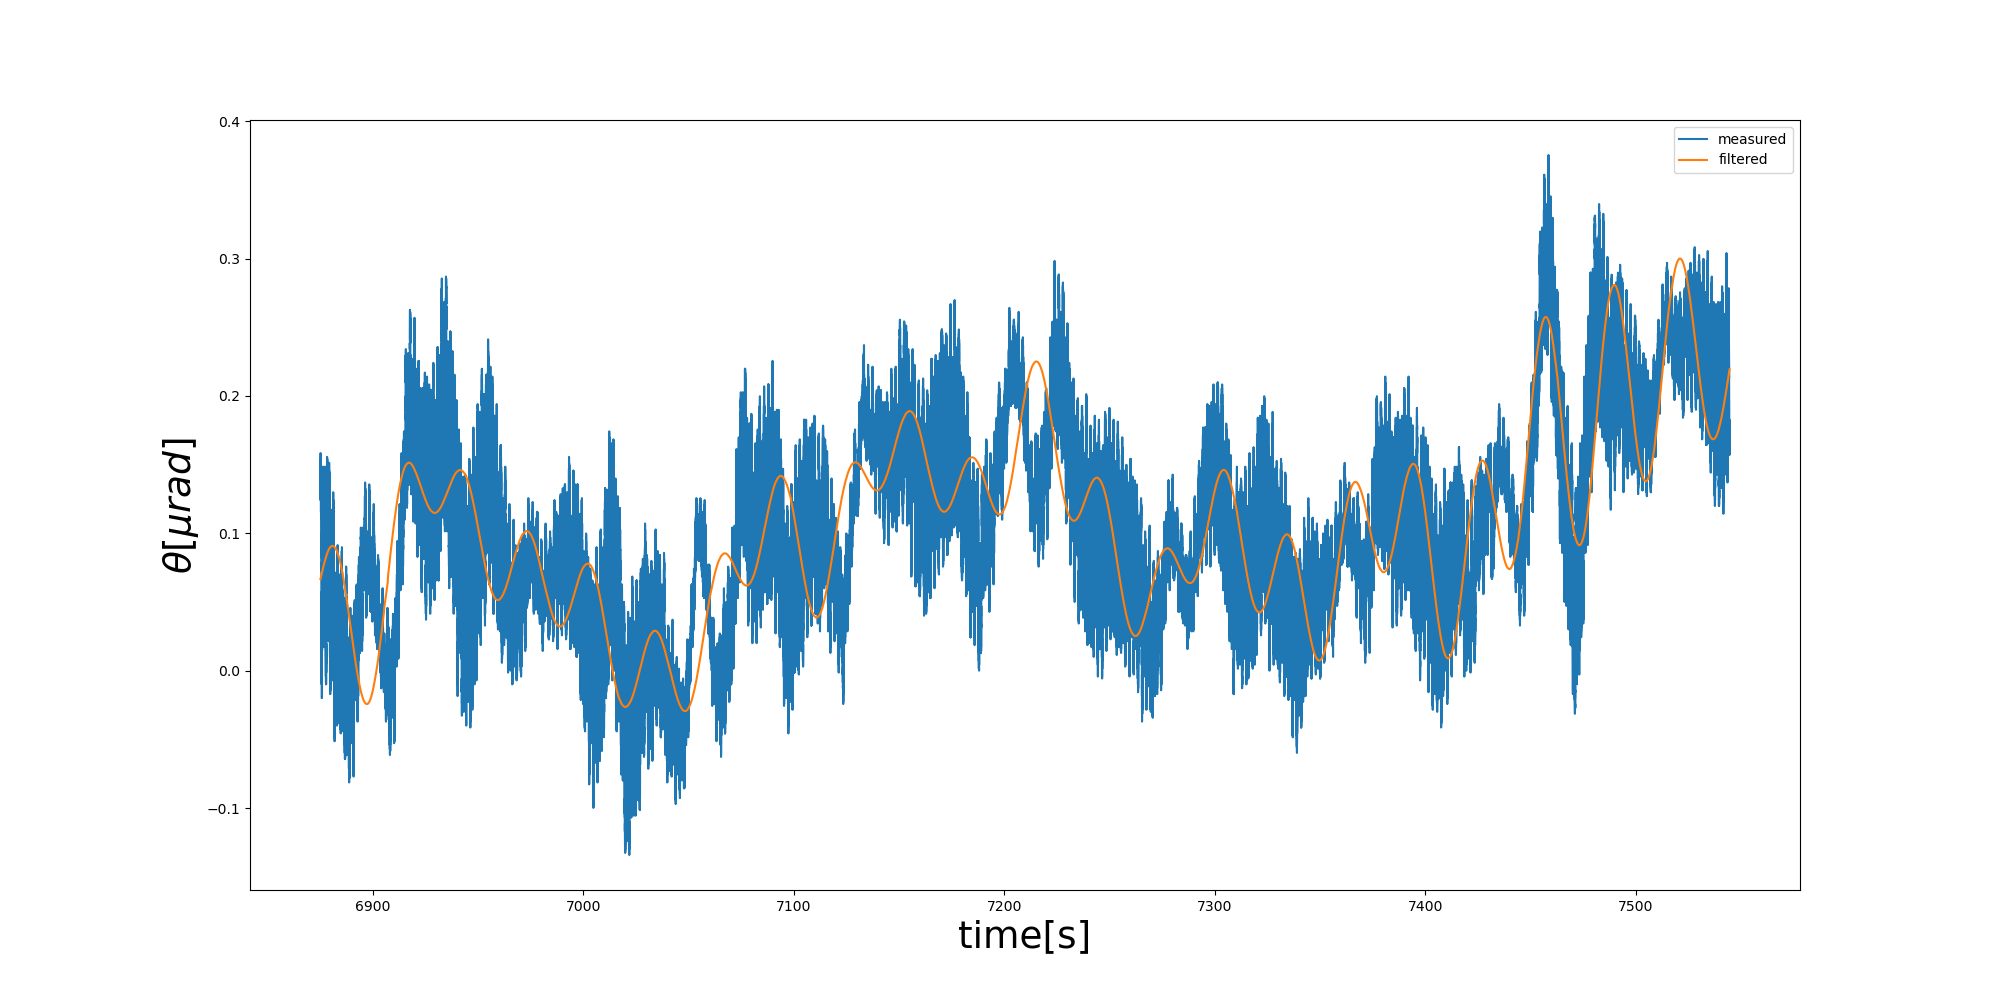
\includegraphics[scale=0.17]{\main/images/4 - methods and results/measured oscillation angle1.png}}
	\caption[The torsional pendulum minimal damped angle]{The torsional pendulum minimal damped angle}
	\label{fig:measured oscillation angle 1}
\end{figure}

Shown in fig.~\ref{fig:measured oscillation angle} are the damped torsional pendulum oscillations, using the PID. Since the damping is depended on the amplitude size (eq.~\ref{eqn:pid damping coefficient}), the damping accelerates as the amplitude gets smaller. 
\par\noindent
Due to PID tourqe power, noise, phase delay (from filtering other modes of the torsional pendulum), and not having the right tuning parameters (which are achieved experimentally), PID is able to damp up to $\theta_{max}\approx 5\cdot 10^{-8}[rad]$.
\par\noindent
Shown in fig.~\ref{fig:measured oscillation angle1} is the minimal average amplitude kept by the PID over time, $\overline{\theta_{max}}\approx 2\cdot 10^{-7}[rad]$. Having a constant amplitude over time, enables to integrate over the results, and have gravitational measurements of..
\par\noindent
\subsection{Quality factor (Q)}
Quality factor ($Q$) is a dimensionless parameter describing how underdamped is the oscillator, it is defined as the ratio of the maximum energy stored in the oscillator to the energy dissipated per cycle of oscillation.
Assuming negligible friction, the energy lost in one cycle is the work done at the cycle, which is the difference between the PID work and the environment noise power $p$ coupled to the oscillator at the cycle (which is independent of time). The work $W_T$ is given by:
\begin{equation}
W_T = \int_0^T[\tau_{PID}(t)\cdot\dot{\theta}(t) - p]dt = \int_0^T\frac{\tau_{max} }{\theta_{max}} \frac{ T}{2\pi}(\frac{2\pi}{T}\theta_{max})^2 sin(\frac{2\pi}{T}t)dt-p\int_0^T dt 
\label{eqn:pid work 1}
\end{equation}
\begin{equation}
W_T = \frac{\tau_{max}\theta_{max}2\pi}{T} \frac{T}{2}-p\cdot T = T\cdot(\frac{\theta_{max}\cdot\pi\tau_{max}}{T} -p)
\label{eqn:pid work}
\end{equation}
The torsional pendulum maximum stored energy in a given cycle $U_T$ is:
\begin{equation}
U_T = \frac{\kappa\cdot\theta(t)^2}{2}+\frac{I\cdot\dot{\theta}(t)^2}{2} =\frac{\kappa(\theta_{max}cos(\omega\cdot 0))^2}{2}+\frac{I(-\omega\theta_{max}sin(\omega\cdot 0))^2}{2} = \frac{\kappa\theta_{max}^2}{2}
\label{eqn:pendulum energy}
\end{equation}
The torsional pendulum damped by the PID Quality factor is:
\begin{equation}
Q = 2\pi\cdot \frac{U_T}{W_T}= 2\pi\cdot\frac{\frac{\kappa\theta_{max}^2}{2}}{T\cdot(\frac{\theta_{max}\cdot\pi\tau_{max}}{T} -p)} =
\frac{\pi}{T}\cdot\frac{\kappa\theta_{max}^2}{\frac{\theta_{max}\cdot\pi\tau_{max}}{T} -p}
\label{eqn:Q}
\end{equation}
\begin{figure}[htbp]
	\centering
	\fbox{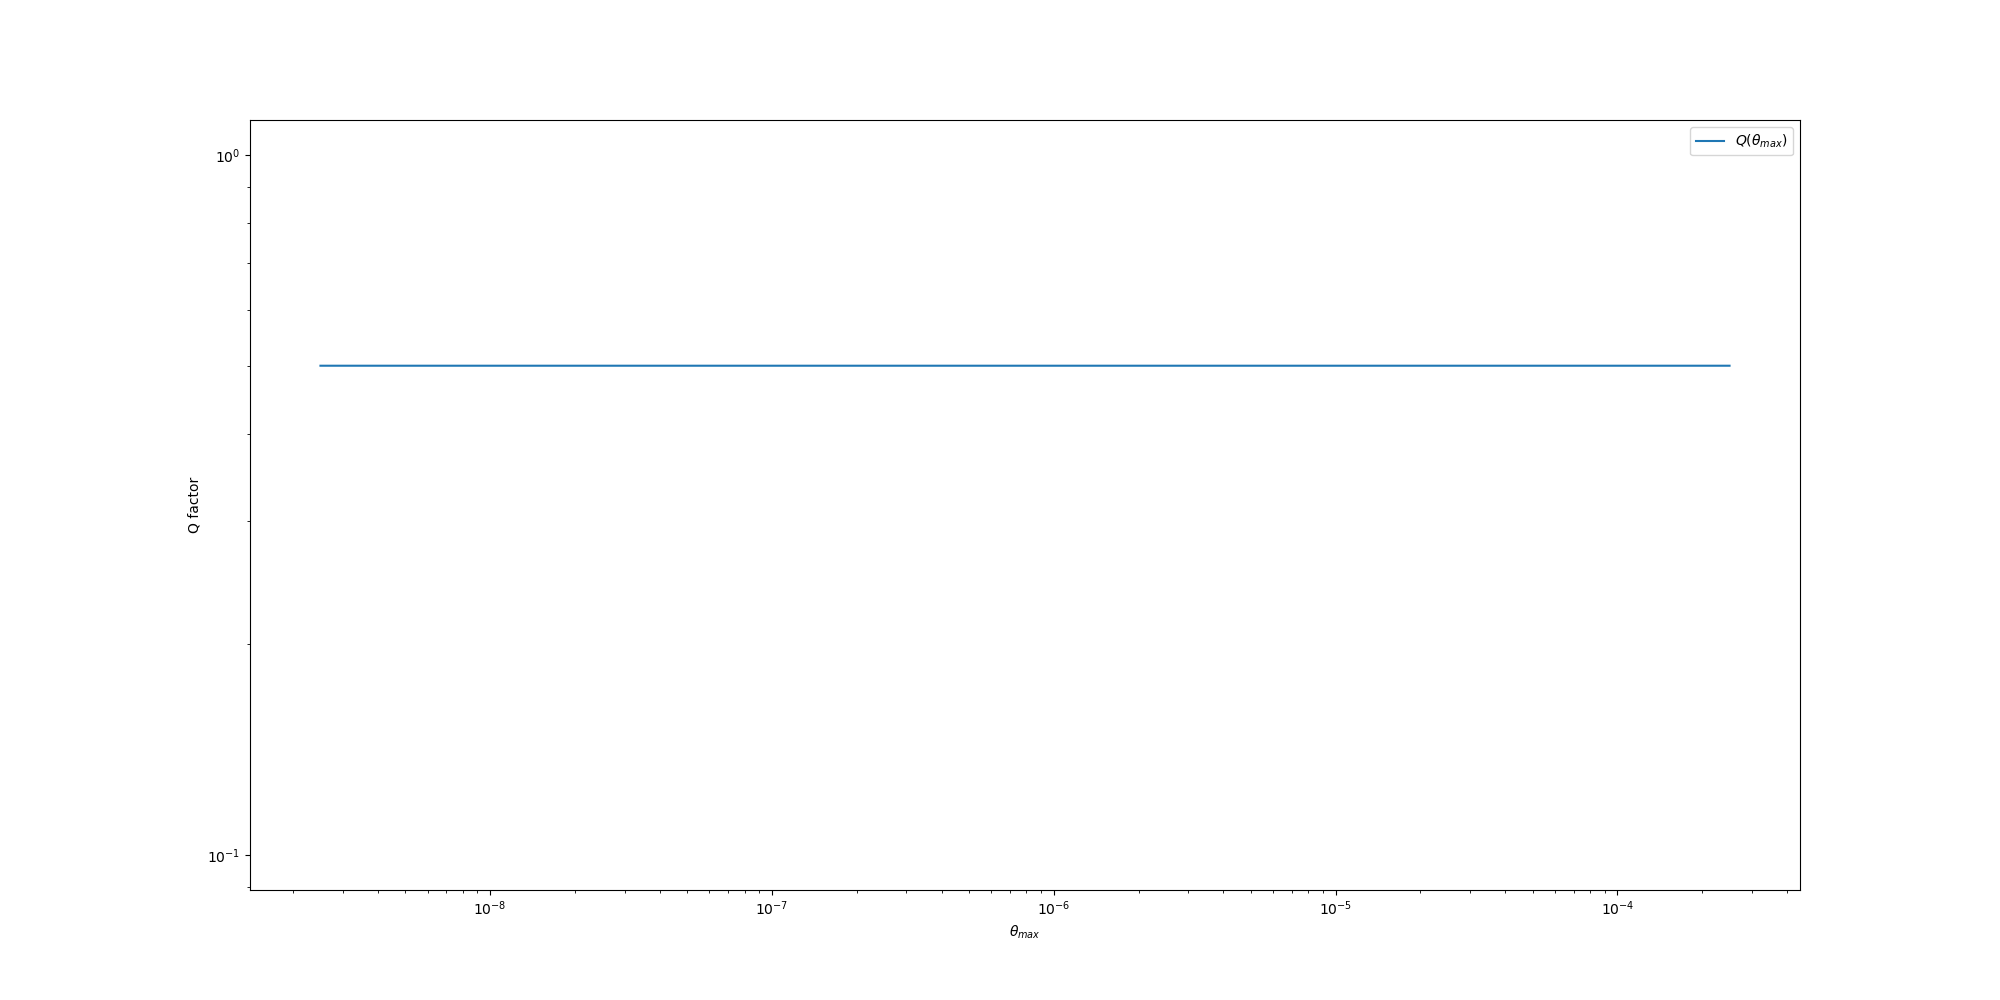
\includegraphics[scale=0.17]{\main/images/4 - methods and results/Q factor.png}}
	\caption[The torsional pendulum Q factor]{The torsional pendulum Q factor}
	\label{fig:Q factor}
\end{figure} 

When $Q>0.5$ the oscillator is underdamped and when $Q>>0.5$ it is highly underdamped. When $Q = 0.5$ the oscillator is critically damped, and when $Q < 0.5$ there is over damping. When Q<0 the noise power coupling is larger than the work done by the PID at the cycle, causing the oscillator to be driven. 
\par\noindent
It can be seen from eq.~\ref{eqn:Q} that the $Q$ factor is highly depended on the oscillation amplitude size $\theta_{max}$. Even when assuming no environmental noises $p=0$, the amplitudes at which the oscillator is not highly underdamped $Q < 1$ (the PID would have effect on the oscillations) are given by:  
\begin{equation}
\theta_{max} < \frac{\tau_{max}}{\kappa} \approx \frac{6.8\cdot 10^{-10}}{2.7\cdot 10^{-6}} \approx 2.5\cdot 10^{-4} [rad]
\label{eqn:low Q}
\end{equation}
From the actual measured angle one can estimate the noises which are introduced to system.




\section{Noise reduction}
As shown previously, there are environment noises affecting the torsional pendulum (eq.~\ref{eqn:Brownian power}, eq.~\ref{eqn:heat conduction}, eq.~\ref{eqn:acoustic power}, eq.~\ref{eqn: Stefan–Boltzmann power}). Assuming gas and environment temperature of $T = 298K$ and pendulum temperature $T_0 = 0K$ (maximal noise power), the noise power is very large. Since the noise energy arrives by particles with random direction and phase the power can be modelled as a Poisson process with the RMS of the number of particles, resulting with a significantly lower effective power $P_{RMS}$.
The RMS of the gas particles number density is $\sqrt{\rho_N} = \sqrt{\frac{P}{k_B T}}$:
\par\noindent
The Brownian effective power is given by:
\begin{equation}
p_{RMS} =   6 A \sqrt{\frac{P}{k_B T}} k_B T  \sqrt{\frac{3RT}{M}}=   6 A T k_B\sqrt{\frac{3 N_A P }{M}}         \label{eqn:RMS Brownian power}
\end{equation}
The maximal thermal effective power is given by: 
\par\noindent
\begin{equation}
p_{RMS} =  A \sqrt{\frac{P}{k_B T}} k_B T c_v  \Delta T \sqrt{\frac{M}{RT}} =  A c_v  \Delta T  \sqrt{\frac{P M }{N_A}}  
\label{eqn:RMS heat conduction}
\end{equation}
The average energy of a black body radiation photon is given by $E=2.7 k_B T$, the maximal black body radiation effective power is given by \cite{WOODS201444}:
\begin{equation}
p_{RMS} = A \cdot\sqrt{N}\cdot E = A\cdot\sqrt{\frac{j}{E}}\cdot E = \sqrt{\frac{\sigma\epsilon(T^4-T_0^4)}{2.7 k_B T}}\cdot 2.7 k_B T A = \sqrt{2.7 k_B T A^2\sigma\epsilon (T^4-T_0^4) }   \label{eqn: max Stefan–Boltzmann power}
\end{equation} 
The noise power is given by:
\par\noindent
\begin{multicols}{2}
\raggedcolumns
\begin{easylist}
& Thermal flow;
&& $p=0.083[W]$.
&& $p_{RMS}=5.33\cdot 10^{-11}[W]$.
& Black body radiation ;
&& $p=0.121[W]$.
&& $p_{RMS}=3.9\cdot 10^{-12}[W]$.
\end{easylist}
\columnbreak
\begin{easylist}
& Brownian motion;
&& $p=0.346[W]$.
&& $p_{RMS}=2.2\cdot 10^{-10}[W]$.
& Acoustic waves;
&& $p=1.14\cdot 10^{-28}[W]$.
\end{easylist}
\end{multicols}

\subsection{Random motion}
Due to random motion, $n_p$ particles collide per second into cross section $A$ of mass $m_1$. Random motion can be modelled as a Poisson process, and the effective collision rate is the square root of the number of events $n_{col} = \sqrt{n_p}$. Each particle exchanges momentum $k$ with with $m_1$, resulting with force $F = n_{col}\cdot k$. Due to the collisions the velosity of $m_1$ is $ u = n_{col}\frac{k}{m_1}$. The collisions result with power given by:
\begin{equation}
p = F\cdot u =  n_{col}k \cdot n_{col}\frac{k}{m_1} =  n_p\frac{ k^2}{m_1}
\label{eqn:net power}
\end{equation}
Due to Brownian motion, there are $n_p= \frac{N}{V}v A$  gas particle collisions with mass $m_0 = \frac{M}{N_A}$ and average velosity of the gas flow $v$ (eq.~\ref{eqn:flow velocity}) collide into $A$. Assuming all collisions are elastic, each particle exchanges momentum of $ k = 2 m_0 v$. Thus, causing Brownian power $p$, which is given by:
\begin{equation}
p =  n_p\frac{ k^2}{m_1} =  \frac{N}{V} v A\frac{ (2 m_0 v)^2}{m_1} = \frac{4AP }{m_1k_B T}(\frac{M}{N_A})^2 (\frac{3 k_B N_A T}{M})^{3/2} =  \frac{12AP }{m_1 } (\frac{3 k_B  T M}{N_A})^{1/2}
\label{eqn:brownian net power}
\end{equation}
Due to environmental black body radiation there are photons colliding into $A$. It can be shown that the mean energy of a black body photon is $E\approx 2.7k_B T$, resulting with $n_p = \frac{j}{E}A$ photon collisions. The incident photons are both absorbed $k_{ab} = \frac{E}{c} $ and reflected $k_{ref} = \frac{2E}{c} $. Thus, causing photon collisions power $p$, which is given by:

\begin{equation}
p =  n_p\frac{ k^2}{m_1} = \frac{j_{ref}}{E}A\cdot\frac{ (\frac{2E}{c})^2}{m_1} +\frac{j_{ab}}{E}A\cdot\frac{ (\frac{E}{c})^2}{m_1} = \frac{ A 2.7 k_B T}{ c^2 m_1} (4j_{ref}+j_{ab}) =\frac{2.7A k_B}{ c^2 m_1} (4-3\epsilon)\sigma T^5 
\label{eqn:photon collision power}
\end{equation}




\end{document}